\chapter{Medición, matrices de densidad y entropía}

El experimento de la doble rendija contiene el problema de la medición en su forma útil más sencilla. Cuando dos alternativas siguen siendo coherentes, sus amplitudes interfieren. Cuando otro sistema adquiere un registro de la alternativa seguida, el objeto y el registrador se entrelazan, y la interferencia cambia. Precisaremos ese mecanismo antes de introducir la traza, la matriz de densidad y la entropía---el lenguaje necesario para cuantificar el entrelazamiento.

\section{Reconstrucción del experimento de la doble rendija}

Consideremos un modelo discreto con una fuente en el sitio \(0\), dos aberturas \(A\) y \(B\), y una pantalla cuyas posibles posiciones de llegada se representan mediante estados ortonormales \(\{|m\rangle\}\). La partícula puede ser un electrón, un fotón o cualquier otro objeto cuántico. La llamaremos electrón y no tendremos en cuenta su espín, de modo que la posición sea el único grado de libertad en cuestión. El resto de la barrera está cerrado: si un electrón llega a cualquier sitio distinto de \(A\) o \(B\), se refleja.

El principio estructural es la linealidad. Si dos estados evolucionan como
\begin{equation}
|A\rangle\longrightarrow |A'\rangle,
\qquad
|B\rangle\longrightarrow |B'\rangle,
\end{equation}
entonces toda superposición evoluciona con los mismos coeficientes:
\begin{equation}
\alpha|A\rangle+\beta|B\rangle
\longrightarrow
\alpha|A'\rangle+\beta|B'\rangle.
\end{equation}

En una disposición simétrica, la fuente alimenta las dos aberturas con la misma amplitud. Omitiendo el factor de normalización común, como en la pizarra,
\begin{equation}
|0\rangle\longrightarrow |A\rangle+|B\rangle.
\end{equation}
El estado normalizado sería \((|A\rangle+|B\rangle)/\sqrt{2}\); el factor omitido no desempeña ningún papel en el argumento sobre la interferencia.

Estudiemos ahora cada trayectoria por separado. La propagación desde las aberturas hasta la pantalla tiene la forma
\begin{align}
|A\rangle &\longrightarrow \sum_m \psi_m|m\rangle, \\
|B\rangle &\longrightarrow \sum_m \phi_m|m\rangle.
\end{align}
El número complejo \(\psi_m\) es la amplitud de llegar a la posición \(m\) de la pantalla partiendo de \(A\), y \(\phi_m\) es la amplitud correspondiente al partir de \(B\).

\begin{figure}[htbp]
\centering
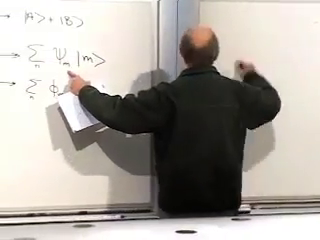
\includegraphics[width=0.68\textwidth]{lecture_07_figure_02.png}
\caption{Las expansiones por separado de las trayectorias \(A\) y \(B\) en la base de la pantalla.}
\lectureframe{00:05:39}
\end{figure}

Si se cierra \(B\), la probabilidad en \(m\) es
\begin{equation}
P_A(m)=|\psi_m|^2.
\end{equation}
Si se cierra \(A\),
\begin{equation}
P_B(m)=|\phi_m|^2.
\end{equation}
La probabilidad clásica sugeriría sumar estas dos respuestas cuando ambas aberturas están disponibles. En cambio, la mecánica cuántica suma primero las amplitudes:
\begin{equation}
|A\rangle+|B\rangle
\longrightarrow
\sum_m(\psi_m+\phi_m)|m\rangle.
\end{equation}
En una posición fija de la pantalla,
\begin{align}
P(m)
&=|\psi_m+\phi_m|^2 \\
&=|\psi_m|^2+|\phi_m|^2
  +\psi_m^*\phi_m+\phi_m^*\psi_m.
\end{align}

\begin{figure}[htbp]
\centering
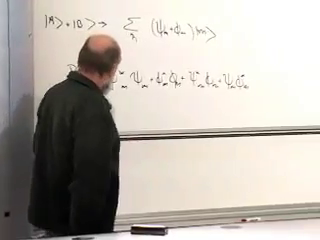
\includegraphics[width=0.70\textwidth]{lecture_07_figure_03.png}
\caption{La probabilidad en la pantalla, con sus cuatro términos. Los dos últimos son los términos de interferencia.}
\lectureframe{00:09:21}
\end{figure}

En un punto de simetría, \(\psi_m=\phi_m\), y las dos alternativas se refuerzan mutuamente. En un punto donde sus fases difieren en \(\pi\), \(\psi_m=-\phi_m\), la probabilidad se anula. Cualquiera de las trayectorias por separado puede llegar a ese punto; sin embargo, abrir ambas puede impedir que el electrón llegue allí. Ahora la pregunta es inevitable: ¿qué cambia cuando algo registra por qué abertura pasó la partícula?

\section{Un detector se entrelaza}

Introduzcamos un sistema auxiliar de dos estados, con estados \(|u\rangle\) y \(|d\rangle\). En este modelo no es el espín del electrón, sino un aparato externo mínimo. Inicialmente, el detector no está activado:
\begin{equation}
|0,d\rangle.
\end{equation}
Dispongamos la interacción de modo que el paso por \(A\) invierta el estado del detector, mientras que el paso por \(B\) lo deje sin cambios:
\begin{equation}
|0,d\rangle
\longrightarrow
|A,u\rangle+|B,d\rangle.
\end{equation}
Una vez que el electrón sale de las aberturas, deja de interactuar con el espín auxiliar. Por tanto, las dos ramas se propagan como
\begin{align}
|A,u\rangle &\longrightarrow \sum_m\psi_m|m,u\rangle, \\
|B,d\rangle &\longrightarrow \sum_m\phi_m|m,d\rangle,
\end{align}
y el estado final es
\begin{equation}
|\Psi\rangle
=\sum_m\left(\psi_m|m,u\rangle+\phi_m|m,d\rangle\right).
\end{equation}
La trayectoria y el registro del detector están ahora entrelazados. Si se lee el detector, se sabrá por qué abertura pasó la partícula.

\begin{classroomqa}
\lecturetimestamp{00:13:24}
\audiencequestion{¿Ya colapsó la función de onda cuando se invierte el espín?}
\lecturerresponse{Si se considera solo el electrón, puede hablarse de colapso: las alternativas de trayectoria ya no interfieren. Sin embargo, en el sistema completo formado por el electrón--detector no se ha descartado ninguna de las ramas. El estado sigue siendo \(|A,u\rangle+|B,d\rangle\). Al incluir el aparato, la afirmación \emph{el electrón colapsó} se sustituye por la afirmación precisa de que se estableció el entrelazamiento entre el sistema--aparato.}
\end{classroomqa}

El espín auxiliar es solo un puntero conveniente. Un dispositivo activado o sin activar, un fotón emitido o ausente, o cualquier otro par de registros distinguibles puede cumplir la misma función.

\begin{classroomqa}
\lecturetimestamp{00:15:17}
\audiencequestion{¿El paso por la placa metálica deja siempre un registro de la trayectoria?}
\lecturerresponse{No necesariamente. Lo que importa es si la interacción deja la placa en estados finales distinguibles. Si la placa tiene una brecha de excitación y el electrón no cuenta con energía suficiente para excitarla, puede que no quede ninguna marca interna duradera. La mera interacción no basta: las dos alternativas deben quedar correlacionadas con registros distinguibles.}
\end{classroomqa}

\begin{classroomqa}
\lecturetimestamp{00:16:29}
\audiencequestion{¿Podría el retroceso de la placa revelar si el electrón pasó por la abertura superior o por la inferior?}
\lecturerresponse{Solo si los impulsos de momento opuestos producen estados de la placa suficientemente distinguibles. Una placa bien localizada ya tiene una función de onda de momento ancha. Los pequeños desplazamientos hacia arriba y hacia abajo pueden solaparse casi por completo, de modo que los estados de retroceso no son ortogonales y no proporcionan un registro inequívoco de la trayectoria. Aquí es donde el principio de incertidumbre protege la interferencia.}
\end{classroomqa}

Es posible un registro parcial. Si el detector recibe solo un impulso pequeño, los dos estados finales del registro no tienen por qué ser ortogonales. En ese caso, la interferencia se reduce, pero no desaparece. Para el cálculo formal, primero consideramos el caso límite de una medición completa:
\begin{equation}
\langle u|d\rangle=0.
\end{equation}

\section{El cálculo con proyectores}

Calculemos ahora la probabilidad de que el electrón llegue a una posición fija \(m\) de la pantalla, sin preguntar cuál fue el resultado del detector. En el espacio de Hilbert combinado, la propiedad \emph{electrón en \(m\)} es un subespacio bidimensional generado por
\begin{equation}
|m,u\rangle,\qquad |m,d\rangle.
\end{equation}
El proyector correspondiente es
\begin{equation}
\Pi_m
=|m,u\rangle\langle m,u|
 +|m,d\rangle\langle m,d|.
\end{equation}

\begin{figure}[htbp]
\centering
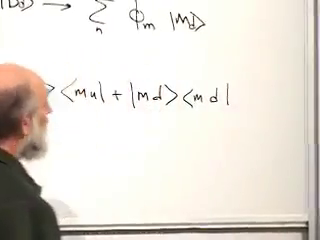
\includegraphics[width=0.66\textwidth]{lecture_07_figure_04.png}
\caption{El proyector sobre una posición fija de la pantalla, sumado sobre los dos registros ortogonales del detector.}
\lectureframe{00:22:04}
\end{figure}

El postulado de probabilidad da
\begin{equation}
P(m)=\langle\Psi|\Pi_m|\Psi\rangle.
\end{equation}
Escribiendo las sumas de forma explícita,
\begin{align}
P(m)
&=
\sum_{n,n'}
\left(\psi_n^*\langle n,u|+\phi_n^*\langle n,d|\right)
\notag\\
&\quad\times\Pi_m
\notag\\
&\quad\times
\left(\psi_{n'}|n',u\rangle+\phi_{n'}|n',d\rangle\right).
\end{align}
Los productos internos de posición exigen que \(n=m=n'\). Luego, los productos internos del detector determinan qué términos permanecen:
\begin{align}
\langle u|u\rangle&=1,
&
\langle d|d\rangle&=1,
&
\langle u|d\rangle&=\langle d|u\rangle=0.
\end{align}
En consecuencia,
\begin{equation}
P(m)=|\psi_m|^2+|\phi_m|^2.
\end{equation}

Los términos cruzados no se han eliminado por decreto. Se anulan porque las dos amplitudes de trayectoria multiplican ahora vectores ortogonales del espacio de estados ampliado. Para que haya interferencia, las alternativas deben coincidir no solo en el punto de llegada a la pantalla, sino también en todos los grados de libertad que llevan un registro.

\section{¿Qué cuenta como medición?}

El modelo sencillo con espín proporciona una regla general: hay medición cuando una interacción establece una correlación entre las alternativas del sistema y estados distinguibles de un aparato. Las siguientes variantes ponen a prueba esa regla.

\begin{classroomqa}
\lecturetimestamp{00:26:53}
\audiencequestion{¿Qué ocurre si el espín se coloca simétricamente y se invierte al pasar por cualquiera de las aberturas?}
\lecturerresponse{Entonces ambas ramas llevan el mismo registro, \(|A,u\rangle+|B,u\rangle=(|A\rangle+|B\rangle)\otimes|u\rangle\). El estado del detector se factoriza y no revela información sobre la trayectoria, por lo que el patrón de interferencia se mantiene.}
\end{classroomqa}

\begin{figure}[htbp]
\centering
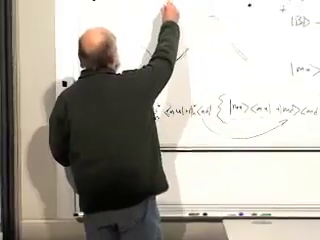
\includegraphics[width=0.68\textwidth]{lecture_07_figure_05.png}
\caption{La variante de la pizarra en la que un detector colocado simétricamente responde igual a ambas trayectorias.}
\lectureframe{00:27:14}
\end{figure}

\begin{figure}[htbp]
\centering
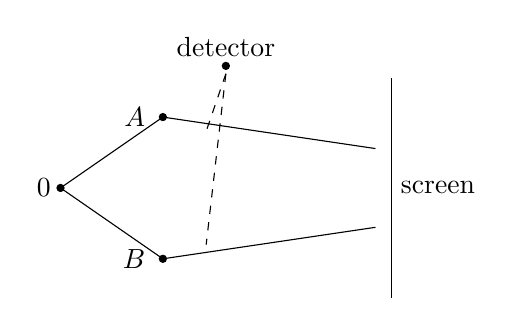
\begin{tikzpicture}[scale=1.0]
\fill (-2,0) circle (1.5pt);
\node[left] at (-2,0) {$0$};
\fill (-0.7,0.9) circle (1.5pt);
\node[left] at (-0.8,0.9) {$A$};
\fill (-0.7,-0.9) circle (1.5pt);
\node[left] at (-0.8,-0.9) {$B$};
\draw (-2,0) -- (-0.7,0.9);
\draw (-2,0) -- (-0.7,-0.9);
\draw (-0.7,0.9) -- (2.0,0.5);
\draw (-0.7,-0.9) -- (2.0,-0.5);
\draw (2.2,-1.4) -- (2.2,1.4);
\node[right] at (2.2,0) {screen};
\fill (0.1,1.55) circle (1.5pt);
\node[above] at (0.1,1.55) {detector};
\draw[dashed] (0.1,1.45) -- (-0.15,0.72);
\draw[dashed] (0.1,1.45) -- (-0.15,-0.72);
\end{tikzpicture}
\caption{Una reconstrucción clara de la disposición simétrica del detector: ambas trayectorias producen el mismo estado del detector.}
\end{figure}

\begin{classroomqa}
\lecturetimestamp{00:27:55}
\audiencequestion{¿Alguien tiene que leer efectivamente el espín auxiliar para que desaparezca la interferencia?}
\lecturerresponse{No. El electrón ya ha correlacionado su trayectoria con el espín. Se puede reiniciar el detector, repetir el experimento con un electrón cada vez e inspeccionar únicamente la distribución de impactos en la pantalla. Las franjas no aparecen aunque nadie lea el espín: lo que importa es el registro físico, no que una persona sea consciente de él.}
\end{classroomqa}

\begin{classroomqa}
\lecturetimestamp{00:29:36}
\audiencequestion{¿Una placa con suficiente poco peso, cuyo retroceso se mida, destruiría la interferencia?}
\lecturerresponse{Sí, si el retroceso desplaza la placa a estados de momento ortogonales para las dos trayectorias. Si los paquetes de onda desplazados todavía se solapan, la destrucción es solo parcial. La masa por sí sola no es el criterio: lo es la distinguibilidad de los estados finales de la placa.}
\end{classroomqa}

La radiación ofrece otro registrador imperfecto. Una partícula cargada acelerada puede emitir un fotón. La radiación emitida cerca de \(A\) no tiene por qué estar en el mismo estado que la emitida cerca de \(B\), por lo que el campo electromagnético puede conservar información sobre la trayectoria. La probabilidad de emisión puede ser pequeña para un electrón desviado lentamente; la clase presenta una estimación ilustrativa de alrededor de un suceso entre cien. Una aceleración mayor hace más probable la emisión de radiación y, por tanto, la pérdida de contraste. El punto importante es cualitativo: incluso un fotón no observado puede llevarse la coherencia.

\begin{classroomqa}
\lecturetimestamp{00:32:00}
\audiencequestion{¿Cómo se infiere la probabilidad de interferencia en un experimento real con contraste imperfecto?}
\lecturerresponse{Se repite el experimento muchas veces y se estima la distribución en la pantalla a partir de las frecuencias relativas. Las muestras finitas y los registros ambientales dejan impactos residuales en regiones nominalmente oscuras. La distribución de probabilidad inferida mejora al aumentar el número de ensayos, mientras que los procesos de decoherencia reducen el contraste físico de las franjas.}
\end{classroomqa}

\begin{classroomqa}
\lecturetimestamp{00:33:13}
\audiencequestion{¿Cualquier posibilidad de determinar la trayectoria destruye toda la interferencia?}
\lecturerresponse{La distinguibilidad completa la destruye por completo. La información parcial produce una pérdida parcial. Un detector que solo gira un poco deja dos estados de registro no ortogonales; por tanto, al leer el detector, una trayectoria resulta más probable que la otra, pero no segura. De forma correspondiente, las franjas se difuminan en vez de borrarse.}
\end{classroomqa}

Sean \(|E_A\rangle\) y \(|E_B\rangle\) estados de registro arbitrarios. El estado combinado en la pantalla puede escribirse
\begin{equation}
|\Psi\rangle
=\sum_m\left(
\psi_m|m\rangle|E_A\rangle
+\phi_m|m\rangle|E_B\rangle
\right).
\end{equation}
Al ignorar el sistema de registro se obtiene
\begin{align}
P(m)
&=|\psi_m|^2+|\phi_m|^2 \\
&\quad
+\psi_m^*\phi_m\langle E_A|E_B\rangle
+\phi_m^*\psi_m\langle E_B|E_A\rangle.
\end{align}
Así, el solapamiento \(\langle E_A|E_B\rangle\) es el factor de coherencia. Los registros idénticos conservan toda la interferencia; los ortogonales la eliminan; un solapamiento intermedio da una visibilidad intermedia.

\begin{classroomqa}
\lecturetimestamp{00:34:12}
\audiencequestion{Si los fotones se emiten solo de vez en cuando, ¿qué ocurre si se consideran únicamente los sucesos en los que se emitió un fotón?}
\lecturerresponse{En general, ese subensamble seleccionado presenta una interferencia menor, porque un fotón lleva información sobre la trayectoria. La pérdida no tiene por qué ser completa: los paquetes de onda de los fotones emitidos en las dos aberturas pueden solaparse, de modo que ni siquiera los registros radiativos son necesariamente perfectamente ortogonales.}
\end{classroomqa}

El bombardeo ambiental amplifica este mecanismo. Las moléculas de aire, los fotones del entorno y la materia circundante adquieren continuamente registros de posiciones macroscópicas. Una persona o la Luna no permanecen visiblemente extendidas en una superposición coherente de posiciones: la masa ralentiza la expansión libre y el entrelazamiento continuo con el entorno suprime la interferencia observable entre alternativas macroscópicamente separadas.

\begin{classroomqa}
\lecturetimestamp{00:36:02}
\audiencequestion{¿Es esto ya una teoría de la medición, y no solo otro uso de la expresión \emph{colapso del paquete de ondas}?}
\lecturerresponse{Es el mecanismo en un ejemplo deliberadamente exacto. En una descripción que considera solo el electrón, colapsar significa descartar los términos no diagonales \(\psi^*\phi\). En la descripción compuesta no hace falta ninguna eliminación ad hoc: el entrelazamiento con estados ortogonales del aparato hace que esos términos no estén disponibles para las mediciones realizadas únicamente sobre el electrón. Los ejemplos más complejos deben remitirse a esta estructura.}
\end{classroomqa}

\begin{classroomqa}
\lecturetimestamp{00:38:04}
\audiencequestion{¿Cambiarían de forma natural el argumento sobre la radiación o la regla de interferencia si un campo gravitatorio curvase la trayectoria?}
\lecturerresponse{La radiación concreta podría cambiar, y la mecánica cuántica no asigna una trayectoria única y bien definida antes de medir el camino. La conclusión general no cambia: solo un grado de libertad que conserve información distinguible sobre la trayectoria suprime la interferencia. Para que una respuesta más detallada tenga sentido, hay que especificar un aparato concreto.}
\end{classroomqa}

\begin{classroomqa}
\lecturetimestamp{00:39:44}
\audiencequestion{¿Esta interferencia es distinta de la interferencia de las ondas electromagnéticas clásicas?}
\lecturerresponse{Para muchos fotones, el patrón observado coincide con la interferencia ondulatoria ordinaria del campo electromagnético. El experimento con una sola partícula muestra la afirmación cuántica más profunda: los fotones y los electrones llegan como sucesos individuales, mientras que sus amplitudes cuánticas interfieren. En el caso de los electrones, la onda pertinente es la función de onda del electrón, no una onda electromagnética.}
\end{classroomqa}

\begin{classroomqa}
\lecturetimestamp{00:40:45}
\audiencequestion{¿Qué ocurre con las partes de la onda inicial dirigidas entre \(A\) y \(B\)?}
\lecturerresponse{En este modelo deliberadamente discreto, el resto de la barrera está bloqueado. Esas partes se reflejan y no contribuyen a la amplitud transmitida en la pantalla. El modelo aísla las dos alternativas transmitidas sin afirmar que un haz real tenga solo dos componentes de momento.}
\end{classroomqa}

\section{El gato, la pantalla y la división móvil}

Las mismas matemáticas se aplican al gato de Schr\"odinger. Sean los estados \(|U\rangle\) y \(|F\rangle\) los del arma sin disparar y disparada, y sean \(|L\rangle\) y \(|D\rangle\) los estados del gato vivo y muerto. Si se parte de un gato vivo y un arma sin disparar, la interacción puede producir
\begin{equation}
|\Psi_{\mathrm{cat}}\rangle
=\alpha|L,U\rangle+\beta|D,F\rangle.
\end{equation}
El gato por sí solo no está en el estado coherente \(\alpha|L\rangle+\beta|D\rangle\). Está entrelazado con un arma que ha registrado la alternativa. Mirar el arma puede revelar la rama del gato, y los registros ortogonales del arma eliminan la interferencia ordinaria entre vivo--muerto en el subsistema del gato.

\begin{classroomqa}
\lecturetimestamp{00:41:18}
\audiencequestion{¿Está el gato mismo en una superposición de vivo y muerto?}
\lecturerresponse{No en el sentido sencillo de un sistema aislado. El sistema compuesto gato--arma está en una superposición de alternativas correlacionadas: vivo con el arma sin disparar y muerto con el arma disparada. El subsistema del gato está entrelazado con un arma que lleva un registro, exactamente como la trayectoria del electrón está entrelazada con el espín auxiliar.}
\end{classroomqa}

La pantalla final también debe tratarse como un aparato. Un electrón que llega a \(m\) puede ennegrecer un grano fotográfico, hacer que un centelleador emita un fotón o invertir uno de los detectores locales de dos estados dispuestos en una fila. La marca queda correlacionada con la posición de llegada.

\begin{classroomqa}
\lecturetimestamp{00:43:38}
\audiencequestion{¿Por qué podemos hablar de probabilidades en la pantalla final en vez de limitarnos a usar vectores de estado indefinidamente?}
\lecturerresponse{El postulado de probabilidad asigna \(\langle\Pi_m\rangle\) a la propiedad \emph{llegada a \(m\)}. Para completar el experimento físico, la pantalla deja después un registro de la posición. El proyector da la probabilidad; el ennegrecimiento, el centelleo o la inversión de un detector local realizan la medición cuyas estadísticas se recopilan.}
\end{classroomqa}

\begin{classroomqa}
\lecturetimestamp{00:45:00}
\audiencequestion{¿Por qué hablamos de una medición en la pantalla, pero no de una probabilidad de paso por \(A\) o \(B\)?}
\lecturerresponse{Solo se pueden asignar y comprobar probabilidades de trayectoria instalando un registrador de trayectorias. Sin ese registro, las alternativas siguen siendo coherentes y deben sumarse como amplitudes. En la pantalla se presupone un aparato sensible a la posición. La diferencia no radica en un instante privilegiado, sino en si se ha dispuesto la interacción de medición correspondiente.}
\end{classroomqa}

La frontera entre el sistema y el aparato puede desplazarse. Incluyamos un observador con estados de registro \(|O_u\rangle\) y \(|O_d\rangle\); entonces
\begin{equation}
|A,u\rangle+|B,d\rangle
\longrightarrow
|A,u,O_u\rangle+|B,d,O_d\rangle.
\end{equation}
A su vez, otro observador puede quedar correlacionado con el primero. El humo en la caja del gato, el arma, el gato, Schr\"odinger y Wigner pueden incluirse todos en una única cadena de entrelazamiento más larga. Sea cual sea la ubicación de la división, las correlaciones deben seguir siendo coherentes: si más tarde Wigner pregunta Schr\"odinger qué vio, sus registros coincidirán.

\begin{classroomqa}
\lecturetimestamp{00:47:24}
\audiencequestion{¿Dónde termina exactamente el sistema y empieza el observador que mide?}
\lecturerresponse{La mecánica cuántica no selecciona una única división conveniente. Se puede hacer colapsar la descripción que considera solo el electrón, incluir el detector y hacer colapsar una descripción más amplia, o incluir un observador y volver a ampliar el estado entrelazado. El requisito físico es que todas las probabilidades y registros accesibles sean coherentes, no que exista una única frontera contable.}
\end{classroomqa}

\begin{classroomqa}
\lecturetimestamp{00:49:47}
\audiencequestion{¿Interviene el principio de incertidumbre porque medir la trayectoria perturba el suceso?}
\lecturerresponse{Sí. El ejemplo del retroceso muestra explícitamente la conexión: localizar la placa produce incertidumbre en el momento, lo cual puede impedir que pequeños impulsos dependientes de la trayectoria se vuelvan distinguibles. En general, una medición cuántica no está completa hasta que el entrelazamiento entre el sistema--aparato ha cambiado el estado, y ese cambio puede alterar la interferencia posterior.}
\end{classroomqa}

Esto marca un contraste claro con el ideal clásico. Clásicamente, se imagina que una medición puede hacerse con una suavidad arbitraria, extrayendo información con una perturbación insignificante. Aquí, extraer información sobre la trayectoria exige establecer una correlación con un aparato. Eso cambia realmente el estado conjunto y altera el resultado de un experimento de interferencia posterior.

\begin{classroomqa}
\lecturetimestamp{00:52:06}
\audiencequestion{¿Qué ocurre si la separación entre \(A\) y \(B\) se hace muy grande?}
\lecturerresponse{No hay una regla nueva universal. En esta geometría de fuente y barrera, las amplitudes de llegar a aberturas muy distantes pueden simplemente volverse pequeñas, de modo que la mayoría de las partículas chocan con la región bloqueada. Aparte de esos cambios, dependientes del aparato, en \(\psi_m\) y \(\phi_m\), la separación por sí sola no determina si se conserva la coherencia.}
\end{classroomqa}

\begin{classroomqa}
\lecturetimestamp{00:53:04}
\audiencequestion{¿Es fundamentalmente exacta la linealidad de la evolución cuántica, y por qué la naturaleza la utiliza?}
\lecturerresponse{La linealidad es un fundamento empírico de la mecánica cuántica. Las pequeñas modificaciones no lineales son notoriamente difíciles de hacer coherentes desde el punto de vista lógico y tienden a estropear la estructura. Aquí no se da la razón más profunda por la que las proposiciones físicas siguen la lógica de los subespacios en vez de la de los conjuntos clásicos; la clase la trata como un hecho de la naturaleza.}
\end{classroomqa}

\begin{classroomqa}
\lecturetimestamp{00:54:53}
\audiencequestion{¿Podría una observación posterior revelar la trayectoria anterior y cambiar así si hubo interferencia?}
\lecturerresponse{Si una observación posterior puede revelar la trayectoria, algún grado de libertad físico debe haber conservado un registro dependiente de ella. Ese registro ya afecta a la coherencia; nadie tiene que leerlo. Aun así, debe respetarse la causalidad, y no se puede resolver una afirmación abstracta sobre elección retardada sin especificar la disposición completa del aparato en el espacio-tiempo.}
\end{classroomqa}

\begin{classroomqa}
\lecturetimestamp{00:56:47}
\audiencequestion{¿Qué ocurriría si se colocara una cámara de burbujas inmediatamente después de las aberturas?}
\lecturerresponse{Una trayectoria que distinga los dos caminos emergentes es una marca inequívoca, por lo que destruye su interferencia. Basta con una capa delgada que registre la trayectoria. Si un dispositivo situado más adelante no conserva información suficiente para inferir por qué abertura pasó antes la partícula, no sirve automáticamente como detector de trayectoria.}
\end{classroomqa}

\begin{classroomqa}
\lecturetimestamp{00:59:29}
\audiencequestion{Si el mundo ya está muy entrelazado, ¿cómo puede empezar un experimento de interferencia con sistemas desenlazados?}
\lecturerresponse{La preparación debe aislar, reiniciar o seleccionar las condiciones de los grados de libertad pertinentes lo suficiente para que las alternativas comiencen con el mismo registro ambiental. No se puede ignorar sin más la trayectoria previa en una cámara de burbujas si sigue correlacionada con el camino. La interferencia requiere una relación inicial aproximadamente factorizada entre el sistema controlado y el registrador pertinente.}
\end{classroomqa}

\begin{classroomqa}
\lecturetimestamp{01:01:04}
\audiencequestion{¿De dónde viene el desenlazamiento práctico después de una medición?}
\lecturerresponse{Condiciónese a un resultado observado definido. Si se encuentra que el espín está hacia arriba, el observador conserva la rama \(|A,u\rangle\) y descarta la alternativa de su descripción de trabajo. Ese estado producto condicionado puede usarse como nuevo punto de partida. El estado completo que incluye al observador puede seguir entrelazado, pero, respecto del resultado registrado, la preparación seleccionada es definida.}
\end{classroomqa}

Esta jerarquía anidada no resuelve todas las cuestiones interpretativas, pero hace visible la coherencia operativa. Se pueden incluir el sistema, el detector, el observador y el observador del observador. Sea cual sea el punto en que se corte la descripción, los registros correctamente correlacionados no se contradicen más adelante.

\section{Del entrelazamiento a la entropía}

La discusión se ha adentrado en la medición más de lo previsto, pero ha puesto de manifiesto la siguiente pregunta: ¿cómo se puede medir el grado de entrelazamiento? Dos espines en el estado producto
\begin{equation}
|u\rangle\otimes|u\rangle
\end{equation}
no están entrelazados. Cada subsistema tiene su propio estado definido, y observar uno no aporta información nueva sobre el otro. Los estados entrelazados no se factorizan de esta manera. Una medida cuantitativa habitual será la entropía de entrelazamiento, pero primero necesitamos la noción ordinaria de entropía y luego su versión cuántica.

\section{La entropía clásica como información faltante}

Empecemos con un sistema clásico que tenga un conjunto finito de \(N\) estados posibles. En este caso, la entropía es una propiedad del sistema junto con nuestro conocimiento de él. Supongamos que lo único que sabemos es que el sistema ocupa uno de \(n\) estados equiprobables. Entonces
\begin{equation}
S=\log n.
\end{equation}
Si \(n=1\), se conoce el estado y \(S=0\). Si \(n=N\), no se sabe nada más que el propio espacio de estados y la entropía es máxima, \(S_{\max}=\log N\).

El logaritmo permite sumar las elecciones independientes de sí--no de forma aditiva. Para \(M\) espines clásicos hay \(2^M\) configuraciones, así que
\begin{equation}
\log(2^M)=M\log 2.
\end{equation}
Por tanto, hasta la elección de la base del logaritmo, la entropía cuenta la cantidad de información binaria que falta en la descripción.

Para una distribución de probabilidad general \(p_i\), la definición adecuada es
\begin{equation}
S=-\sum_i p_i\log p_i.
\end{equation}

\begin{classroomqa}
\lecturetimestamp{01:14:17}
\audiencequestion{¿Por qué hay un signo menos en la fórmula de la entropía?}
\lecturerresponse{Toda probabilidad distinta de cero satisface \(0<p_i\leq 1\), de modo que \(\log p_i\leq 0\). El signo menos hace que la entropía sea no negativa. Para \(p_i=0\), la contribución se define mediante el límite \(p_i\log p_i\to0\).}
\end{classroomqa}

Para la distribución equiprobable
\begin{equation}
p_i=
\begin{cases}
1/n, & i\in\mathcal N,\\
0, & i\notin\mathcal N,
\end{cases}
\qquad |\mathcal N|=n,
\end{equation}
la fórmula general se convierte en
\begin{align}
S
&=-n\left(\frac1n\right)\log\left(\frac1n\right)\\
&=\log n.
\end{align}
Por tanto, reproduce la definición elemental por conteo. Una distribución concentrada con certeza en un solo estado tiene \(S=0\).

\begin{figure}[htbp]
\centering
\includegraphics[width=0.66\textwidth]{lecture_07_figure_07.png}
\caption{La pizarra reúne \(S=\log n\), la fórmula de Shannon y la comprobación para probabilidades iguales.}
\lectureframe{01:16:08}
\end{figure}

\begin{classroomqa}
\lecturetimestamp{01:17:35}
\audiencequestion{¿Cuál es la entropía máxima que puede tener un sistema con \(N\) estados, y qué se sabe en ese caso?}
\lecturerresponse{El máximo es \(\log N\), y se alcanza con la distribución uniforme \(p_i=1/N\). Aún se sabe qué es el sistema y, por tanto, cuál es su espacio de estados; lo que se desconoce es cuál de esos \(N\) estados ocupa.}
\end{classroomqa}

La diferencia
\begin{equation}
I=S_{\max}-S
\end{equation}
es la información disponible en este sentido contable. La entropía y la información son dos caras del mismo registro: la entropía refleja la información que podría permitir distinguir el estado, pero que no está a nuestro alcance.

\section{La traza: el reemplazo cuántico de una suma}

Para un operador \(M\) y cualquier base ortonormal completa \(\{|i\rangle\}\), definimos
\begin{equation}
\operatorname{Tr}M
=\sum_i\langle i|M|i\rangle.
\end{equation}

\begin{figure}[htbp]
\centering
\includegraphics[width=0.68\textwidth]{lecture_07_figure_08.png}
\caption{La traza escrita como suma de los elementos diagonales de la matriz.}
\lectureframe{01:21:20}
\end{figure}

Aunque la definición se expresa usando una base, el resultado es independiente de ella. Para un operador hermítico se puede elegir una base de autovectores, en la que
\begin{equation}
\operatorname{Tr}M=\sum_i\lambda_i.
\end{equation}
Los autovalores, y por tanto su suma, no dependen de las coordenadas usadas para representar el operador.

\begin{classroomqa}
\lecturetimestamp{01:23:04}
\audiencequestion{¿Que una matriz esté en forma diagonal implica que tiene inversa?}
\lecturerresponse{No. La forma diagonal muestra los valores propios; la invertibilidad es una condición aparte. Una matriz diagonal es invertible precisamente cuando ninguno de sus valores propios diagonales es cero. Las matrices hermíticas son diagonalizables incluso si algunos valores propios se anulan.}
\end{classroomqa}

Después de la pausa, volvamos brevemente a la probabilidad clásica. Un observable clásico es una función \(f_i\) de la configuración, y su promedio es
\begin{equation}
\langle f\rangle_{\mathrm{cl}}=\sum_i p_i f_i.
\end{equation}
En las fórmulas cuánticas, la traza sustituirá a la suma sobre alternativas, un operador sustituirá a la función clásica y una matriz de densidad sustituirá a la distribución de probabilidad.

\section{Mezclas estadísticas y matriz de densidad}

Supongamos que alguien prepara un sistema en uno de los estados de una base ortonormal, pero no nos dice cuál eligió. Solo proporciona las probabilidades de preparación---; por ejemplo, un espín se prepara hacia arriba con probabilidad \(3/4\) y hacia abajo con probabilidad \(1/4\). Esto no es la superposición coherente
\begin{equation}
\sqrt{\frac34}|u\rangle+\sqrt{\frac14}|d\rangle,
\end{equation}
porque no se ha preparado ninguna fase relativa. Es una mezcla estadística de estados definidos. Las probabilidades cuánticas persisten incluso cuando se conoce un estado puro; aquí hay, además, incertidumbre sobre cuál de los estados puros se preparó.

\begin{figure}[htbp]
\centering
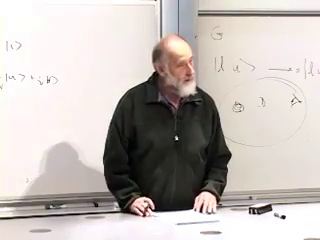
\includegraphics[width=0.66\textwidth]{lecture_07_figure_06.png}
\caption{La transición conceptual de un ket especificado a una descripción de conjunto.}
\lectureframe{01:29:43}
\end{figure}

Si el estado \(|i\rangle\) se prepara con probabilidad \(\rho_i\), el operador densidad es
\begin{equation}
\rho=\sum_i\rho_i|i\rangle\langle i|.
\end{equation}
En la base de preparación,
\begin{equation}
\rho=
\begin{pmatrix}
\rho_1&0&0&\cdots\\
0&\rho_2&0&\cdots\\
0&0&\rho_3&\cdots\\
\vdots&\vdots&\vdots&\ddots
\end{pmatrix}.
\end{equation}

\begin{figure}[htbp]
\centering
\includegraphics[width=0.68\textwidth]{lecture_07_figure_09.png}
\caption{La matriz de densidad diagonal y su condición de normalización.}
\lectureframe{01:32:12}
\end{figure}

Sus valores propios son reales y no negativos, y la normalización de las probabilidades se expresa como
\begin{equation}
\operatorname{Tr}\rho=\sum_i\rho_i=1.
\end{equation}

Sea \(F\) un observable hermítico. El valor esperado del conjunto es
\begin{equation}
\langle F\rangle=\operatorname{Tr}(F\rho).
\end{equation}

\begin{figure}[htbp]
\centering
\includegraphics[width=0.68\textwidth]{lecture_07_figure_10.png}
\caption{El valor esperado expresado mediante la traza, \(\langle F\rangle=\operatorname{Tr}(F\rho)\).}
\lectureframe{01:35:05}
\end{figure}

Para recuperar el promedio ponderado habitual, calculemos la traza en la base en la que \(\rho\) es diagonal e introduzcamos la resolución de la identidad:
\begin{align}
\operatorname{Tr}(F\rho)
&=\sum_i\langle i|F\rho|i\rangle\\
&=\sum_{i,j}\langle i|F|j\rangle
               \langle j|\rho|i\rangle\\
&=\sum_i\rho_i\langle i|F|i\rangle.
\end{align}
Así, cada valor esperado del estado puro queda ponderado por la probabilidad de que se haya preparado el estado correspondiente.

La traza tiene la propiedad cíclica
\begin{equation}
\operatorname{Tr}(AB)=\operatorname{Tr}(BA),
\end{equation}
incluso si \(A\) y \(B\) no conmutan. Por tanto, \(\operatorname{Tr}(F\rho)=\operatorname{Tr}(\rho F)\).

\section{Entropía cuántica y la recompensa aplazada}

La entropía de una matriz de densidad es
\begin{equation}
S(\rho)=-\operatorname{Tr}(\rho\log\rho).
\end{equation}
Para un operador hermítico positivo, las funciones como \(\log\rho\) se definen a partir de sus valores propios. Si
\begin{equation}
\rho=\sum_i\rho_i|i\rangle\langle i|,
\end{equation}
entonces
\begin{equation}
\log\rho=\sum_{\rho_i>0}(\log\rho_i)|i\rangle\langle i|,
\end{equation}
y, por tanto,
\begin{equation}
S(\rho)=-\sum_i\rho_i\log\rho_i.
\end{equation}

\begin{figure}[htbp]
\centering
\includegraphics[width=0.68\textwidth]{lecture_07_figure_11.png}
\caption{La fórmula de la entropía clásica expresada como \(S=-\operatorname{Tr}(\rho\log\rho)\).}
\lectureframe{01:41:25}
\end{figure}

Un estado puro conocido tiene como operador densidad
\begin{equation}
\rho_\psi=|\psi\rangle\langle\psi|,
\end{equation}
con valores propios \(1,0,\ldots\), de modo que \(S(\rho_\psi)=0\). Esto no significa que toda medición sobre \(|\psi\rangle\) tenga un resultado cierto. Significa que no hay ignorancia estadística adicional sobre el estado preparado. En el extremo opuesto,
\begin{equation}
\rho=\frac{I}{d}
\qquad\Longrightarrow\qquad
S(\rho)=\log d,
\end{equation}
donde \(d=\dim\mathcal H\). El estado máximamente mezclado asigna el mismo peso a todas las direcciones ortogonales.

La conexión con el entrelazamiento está cerca, pero aún no la hemos desarrollado. Supongamos que un sistema compuesto \(AB\) está en un estado conjunto y que todos los experimentos se limitan a \(A\). Debe existir un objeto que reproduzca todos los valores esperados que puedan obtenerse en \(A\) cuando se ignora \(B\). Ese objeto es una matriz de densidad para \(A\). Si el estado conjunto se factoriza, la matriz de densidad de \(A\) es pura y tiene entropía nula. Si \(A\) y \(B\) están entrelazados, la matriz de densidad de \(A\) suele ser mixta y tener entropía distinta de cero. Construir esa matriz de densidad reducida y calcular su entropía es la tarea que dejamos para la próxima clase.
